\documentclass[a4paper,12pt]{article}
\usepackage[utf8]{inputenc}
\usepackage[magyar]{babel}
\usepackage{amsmath, amssymb}
\usepackage{enumitem}
\usepackage{multicol}
\usepackage{tikz}
\usetikzlibrary{intersections}
\usetikzlibrary{calc}
\usetikzlibrary{angles}
\usetikzlibrary{turtle}
\usetikzlibrary{backgrounds}
\usepackage{pgfplots}
\pgfplotsset{compat=1.18}
\usepgfplotslibrary{fillbetween}
\usepackage[a4paper, margin=25mm]{geometry} % smaller margins
\setlength{\parindent}{0pt}
\setlength{\parskip}{10pt}
\setlist[itemize]{before=\vspace{-1.5\parskip},after=\vspace{-1.5\parskip}}
\setlist[enumerate]{before=\vspace{-1.5\parskip},after=\vspace{-1.5\parskip}}
\tolerance=10000

% https://github.com/pgf-tikz/pgf/issues/1047
% https://github.com/pgf-tikz/pgf/pull/1316
\usepackage{regexpatch}
\makeatletter
\xpatchcmd*\tikz@foreach
  {\tikz@lastysaved=\tikz@foreach@save@lastysaved}
  {\tikz@lastysaved=\tikz@foreach@save@lastysaved
   \let\tikz@tangent=\tikz@foreach@save@tangent}
  {}{\PatchFailed}

\xpatchcmd*\tikz@foreach
  {\xdef\tikz@foreach@save@lastysaved{\the\tikz@lastysaved}}
  {\xdef\tikz@foreach@save@lastysaved{\the\tikz@lastysaved}%
   \global\let\tikz@foreach@save@tangent=\tikz@tangent}
  {}{\PatchFailed}
\makeatother


\begin{document}

1) Vegyünk egy egységsugarú kört és a beleírt szabályos hatszöget a főátlóival!

%% \begin{center}
%%   \begin{tikzpicture}[scale=3, rotate=30]
%%     \draw (0,0) -- (0,1) node (a) {} \foreach \x in {b,...,f} {-- ([turn] 60:1) node (\x) {}};
%%     \draw (a.center) -- (d.center);
%%     \draw (b.center) -- (e.center);
%%     \draw (c.center) -- (f.center);
%%   \end{tikzpicture}
%% \end{center}

%% \begin{center}
%%   \begin{tikzpicture}[scale=3]
%%     \draw
%%         [turtle=home,right=30]
%%         \foreach \n in {a,...,f} { [turtle={forward,right=60}] node (\n) {} };
%%     \draw (a.center) -- (d.center);
%%     \draw (b.center) -- (e.center);
%%     \draw (c.center) -- (f.center);
%%     \draw (1,0) circle (1);
%%   \end{tikzpicture}
%% \end{center}

%% \begin{center}
%%   \begin{tikzpicture}[scale=3,y=(60:1)]
%%     \draw (0,1) -- (0,2) -- (1,2) -- (2,1) -- (2,0) -- (1,0) -- cycle;
%%     \draw (1,1) [y=1cm] circle (1);
%%     \draw (0,1) -- (2,1);
%%     \draw (0,2) -- (2,0);
%%     \draw (1,0) -- (1,2);
%%   \end{tikzpicture}
%% \end{center}

\begin{center}
  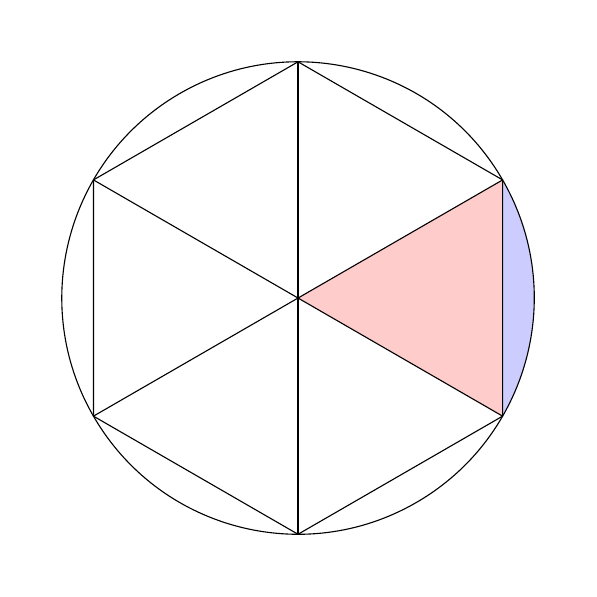
\begin{tikzpicture}[rotate=30,scale=3]
    \begin{scope}[rotate=30, xscale=sqrt(3)/2, yslant=0.5]
      %% \draw[lightgray, very thin] grid (2,2);
      \draw[name path global=hatszog] (0,1) -- (0,2) -- (1,2) -- (2,1) -- (2,0) -- (1,0) -- (0,1);
      \coordinate (center) at (1,1);
      \coordinate (a) at (2,0);
      \coordinate (b) at (1,0);
      \draw (0,1) -- (2,1);
      \draw (0,2) -- (2,0);
      \draw (1,0) -- (1,2);
      \scoped[on background layer] \fill [red!20] (1,1) -- (2,0) -- (1,0);
    \end{scope}
    \draw[name path=kor] (center) circle (1);
    \scoped[on background layer]\fill [blue!20, intersection segments={of=hatszog and kor, sequence= { L0 -- R0 }}];
  \end{tikzpicture}
\end{center}

Az egységsugár azt jelenti, hogy a feladatmegoldás során erre a körre
mindig úgy gondolhatsz, hogy a sugara 1.  Az ábrán látható hatszög
(ami 6 háromszögből áll) minden oldala 1 hosszú.

Határozzuk meg a következőket:

\begin{enumerate}[label=\alph*)]
\item A kör kerületét!
\item A hatszög kerületét!
\item A kör és a hatszög kerületének különbségét! \newline (Számológéppel tudod csak kiszámolni a tizedesjegyek miatt.)
\end{enumerate}

Folytatás a következő oldalon!

\newpage

\def\rajz#1#2#3{
  \begin{center}
    \begin{tikzpicture}[yscale=-1,rotate=-0.5*#2]
      \pgfmathsetmacro{\scale}{#1}
      \pgfmathsetmacro{\angle}{#2}
      \pgfmathsetmacro{\length}{#3}
      \draw (0,0) coordinate (a) node[left]{$A$}
      -- ([turn]90:\scale) coordinate (b) node[right]{$B$}
      -- ([turn]90+0.5*\angle:\scale*\length) coordinate (c) node[below]{$C$}
      -- ([turn]90+0.5*\angle:\scale);
      \path[name path=bc] (b) -- (c);
      \path[name path=felezo] (a) -- (0.5*\angle:\scale);

      %% \draw let \p1 = (x) in (x) node[above right]{(\pgfkeys{/pgf/number format/.cd,precision=3}\pgfmathparse{\x1*1pt/1cm}\pgfmathprintnumber{\pgfmathresult}, \pgfmathparse{\y1*1pt/1cm}\pgfmathprintnumber{\pgfmathresult})};

      \scoped[on background layer] \fill [red!20] (a) -- (b) -- (c);

      \draw (\scale,0) [name path=kor] arc [start angle=0, end angle=\angle, radius=\scale];
      \scoped[on background layer]\fill [blue!20, intersection segments={of=bc and kor}];

      \begin{scope}[green!50!black, very thick]
        \path[name intersections={of=bc and felezo,  by=x}] (x) node[below left] {$X$};
        \path[name intersections={of=felezo and kor, by=y}] (y) node[right     ] {$Y$};

        \draw (a) -- (y);
        \draw (b) -- (y) -- (c);

        \pic [pic text=., angle radius = 3mm, draw] {angle = b--x--a};
        \pic [pic text=., angle radius = 3mm, draw] {angle = y--x--b};
      \end{scope}
    \end{tikzpicture}
  \end{center}
}

2) A hatszöget úgy alakíthatjuk szabályos tizenkétszöggé, hogy minden
háromszögnek behúzzuk a szögfelezőjét a kör közepétől a körig és
ezeket az új metszéspontokat összekötjük a régi hatszög szomszédos
csúcsaival.

Vizsgáljuk meg ezt a módszert az ábra hatodán!

\rajz{10}{60}{1}

A BC szakasz hosszát ismerjük, az a hatszög egy oldala!

Figyelem: az ABY háromszög semmilyen szempontból nem speciális, csak egy
alkotó háromszöge a tizenkétszögnek, egyik szöge sem derékszög.

Határozzuk meg a következőket (ebben a sorrendben, használhatsz számológépet):

\begin{enumerate}[label=\alph*)]
\item Az AY szakasz hosszát! (egyszerű)
\item A BX szakasz hosszát! (egyszerű)
\item Az AX szakasz hosszát!
\item Az XY szakasz hosszát!
\item A BY szakasz hosszát!
\item A tizenkétszög kerületét!
\end{enumerate}

\newpage

3) Az egész számításban sehol nem használtuk ki, hogy 60 fokos szög
helyezkedik el az $A$ csúcsnál, ezért a felezést meg tudjuk ismételni
az új tizenkétszög egy kis háromszögében is!  Egy huszonnégyszög pedig
már majdnem akkora, mint egy kör.

\rajz{14}{30}{0.5176380902050415} % ./pi.py

A felezéseket tetszőlegesen sokáig végezhetjük, minden lépésben
a sokszög szögeinek száma a duplájára nő.  A sokszög kerülete pedig a
kör kerületének egyre jobb közelítését adja.

Az ábrát és az eddig összegyűjtött tudásunkat használva, töltsük ki az
alábbi ``felező'' függvény kérdőjelekkel megjelölt, hiányzó részeit!

A függvény bemeneti értéke egy sokszög oldalhossza és visszaadja az
eljárás szerint készült kétszer olyan sokszög oldalhosszát.

\begin{verbatim}
from math import sqrt

def felezo(BC):
  BX = ???
  AX = ???
  XY = ???
  BY = ???
  return BY
\end{verbatim}

\newpage

4) Írjuk meg a főprogramot, hogy lefuttathassuk az egész programot!

Hiányoznak még a kezdőértékek, ezeket írjuk be az első feladat alapján!

Utána a ciklus a felező függvényt hívva kiírja a kör kerületének egyre
és egyre jobb közelítéseit.

\begin{verbatim}
from math import sqrt

def felezo(BC):
  ...
  return BY

def run():
  BC = ???
  szogszam = ???
  for i in range(20):
    kerulet = BC * szogszam
    print(f"{szogszam:8d}-szög kerülete: {kerulet:.12f}")
    BC = felezo(BC)
    szogszam *= 2

run()
\end{verbatim}

\end{document}
